\begin{figure}[h]
  \begin{center}
    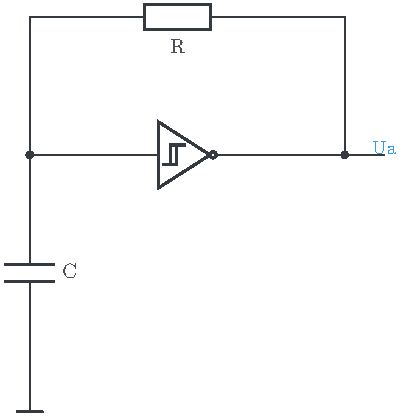
\includegraphics[height=0.382\textwidth]{VBA/4/astabil_schmitt}
  \end{center}
  \caption{Mutlivibratorschaltung mit Schmitt-Trigger}
  \label{fig:astable1}
\end{figure}

Astabile Multivibratoren besitzen keinen stabilen Ausgangszustand, weshalb sie
sich zur Taktgenerierung eignen. Abbildung \ref{fig:astable1} zeigt ein
Beispiel eines astabilen Multivibrators mit einem invertierenden Schmitt-Trigger
und einer RC-Kombination. Da es keinen stabilen Zustand gibt, sollte man zur Analyse einen
der Zustände an den Ausgängen der logischen Gatter annehmen, da diese nur 0 oder
$U_{\mathrm{S}}$ sein können. Ist zum Beispiel der Ausgang des Triggers
\HIGH, lädt sich der Kondensator $C$ über den Widerstand $R$ auf (unter der
Annahme, dass der Strom in/aus Gattereingänge/n vernachlässigbar ist). Erreicht
die Spannung über dem Kondensator (gegen Masse) den oberen Eingangsschwellwert
des Schmitt-Triggers, dann schaltet der Triggerausgang auf \LOW (invertierend).
Der Kondensator entlädt sich nun über $R$ bis die untere
Trigger-Eingangsschwelle erreicht ist und der Ausgang wieder zu \HIGH wird.

Abbildung \ref{fig:astable2} zeigt eine weitere Realisierungsmöglichkeit einer
astabilen Multivibratorschaltung mit zwei Invertern.

\begin{figure}[h]
  \begin{center}
    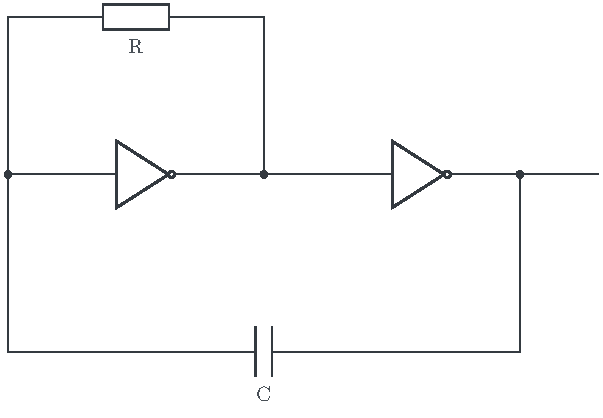
\includegraphics[width=0.618\textwidth]{VBA/4/astabil}
  \end{center}
  \caption{Weitere Möglichkeit einer astabilen Multivibratorschaltung}
  \label{fig:astable2}
\end{figure}

